\documentclass{article}




% This format originated from that of NeurIPS 2023.
\usepackage[preprint,nonatbib]{neurips_2023}



\usepackage[utf8]{inputenc} % allow utf-8 input
\usepackage[T1]{fontenc}    % use 8-bit T1 fonts
\usepackage{url}            % simple URL typesetting
\usepackage{booktabs}       % professional-quality tables
\usepackage{amsfonts}       % blackboard math symbols
\usepackage{amsmath}       % blackboard math symbols
\usepackage{nicefrac}       % compact symbols for 1/2, etc.
\usepackage{microtype}      % microtypography
\usepackage{xcolor}         % colors
\usepackage{graphicx}
\usepackage{hyperref}       % hyperlinks
\usepackage[ruled,vlined,linesnumbered]{algorithm2e}
\usepackage[style=authoryear,backend=bibtex]{biblatex}
\addbibresource{main.bib}

\newcommand{\B}[1]{\mathbf{#1}}
\newcommand{\TB}[1]{\textbf{#1}}
\newcommand{\etal}{\textit{et al}.~}
\newcommand{\robotConfig}{\mathcal{C}}


\title{A Survey of the Applications of Deep Reinforcement 
Learning for Motion Planning \& Control of Unmanned Aerial Vehicles}


% The \author macro works with any number of authors. There are two commands
% used to separate the names and addresses of multiple authors: \And and \AND.
%
% Using \And between authors leaves it to LaTeX to determine where to break the
% lines. Using \AND forces a line break at that point. So, if LaTeX puts 3 of 4
% authors names on the first line, and the last on the second line, try using
% \AND instead of \And before the third author name.


\author{%
  Baozhe Zhang \\
  School of Science and Engineering\\
  The Chinese University of Hong Kong, Shenzhen\\
  \texttt{baozhezhang@link.cuhk.edu.cn} \\
  % examples of more authors
  % \And
  % Coauthor \\
  % Affiliation \\
  % Address \\
  % \texttt{email} \\
  % \AND
  % Coauthor \\
  % Affiliation \\
  % Address \\
  % \texttt{email} \\
  % \And
  % Coauthor \\
  % Affiliation \\
  % Address \\
  % \texttt{email} \\
  % \And
  % Coauthor \\
  % Affiliation \\
  % Address \\
  % \texttt{email} \\
}


\begin{document}


\maketitle


\begin{abstract}
  This survey explores Deep Reinforcement Learning (DRL) in motion planning and control for Unmanned Aerial Vehicles (UAVs). Traditional methods have been the backbone of UAV control and planning, offering precise mathematical models for dynamics and trajectory generation. However, their model-driven nature often results in sub-optimal performance in the stochastic, real-world environment, especially in complex tasks like high-speed drone racing.
  In contrast, DRL, known for its data-driven approach, excels in learning from vast amounts of data and adapting to dynamic environments. This survey highlights key works that demonstrate DRL's ability to overcome limitations of traditional methods, offering unified, scalable, and generalizable frameworks for UAV motion planning and control. 
  The fusion of traditional methods with the data-rich capabilities of DRL is proposed as a future direction, promising to yield more robust and versatile UAV systems.
\end{abstract}


\section{Introduction}
Recently, micro aerial vehicles (MAVs) or 
unmanned Aerial Vehicles (UAVs), commonly known as drones, 
have emerged as a powerful tool in various industries, 
ranging from agriculture and real estate to filmography and delivery 
services. 
Their versatility and cost-effectiveness have led to a 
surge in applications that require multiple drones to operate 
collaboratively. 
Operating in real-world dynamic environments, 
these UAV systems need to navigate a wide range of 
challenges, 
including moving obstacles, inter-drone coordination, and 
real-time adaptability. 



The traditional planning and control pipelines for mobile robots' 
autonomous navigation have been extensively studied in recent
decades in the literature. 
Many complete systems with simultaneous localization 
and mapping (SLAM) and hierarchical 
planning and control frameworks can achieve outstanding 
autonomy.
For example, {\textcite{zhou2019robust}} propose a robust and efficient 
quadrotor motion planning system for fast flight in 
three-dimensional complex environments.
{\textcite{quan2023robust}} introduce a distributed motion planning 
trajectory optimization framework for large-scale quadrotor 
formation flight in dense environments.
Although traditional methods can achieve impressive performance, 
there are limitations and challenges associated with these methods: 
\begin{itemize}
  \item \TB{Complexity}. The hierarchical planning and control 
  methods consist of multiple layers of modules,   
  each of which requires fine-tuning of 
  its parameters, increasing the overall complexity of the system.
  \item \TB{Modeling Limitation}. Traditional methods rely on 
  accurate models of the environment and the system. However, 
  creating precise models, especially for complex systems like 
  drones, can be challenging. Small discrepancies between the 
  model and reality can lead to significant performance 
  degradation. 
  \item \TB{Generalizability}. Many traditional methods are 
  tailored to specific tasks, environments, 
  or robot platforms. Transferring them 
  to new tasks or settings often requires significant 
  modifications. 
\end{itemize}

The capability of the 
classical hierarchical motion planning framework is 
challenged 
as the complexity and randomness of robot application 
scenarios increase. 
Recent advancements in artificial intelligence have fostered 
the development of Deep Reinforcement Learning (DRL) - a branch 
of machine learning that trains agents to make sequential 
decisions by interacting with an environment. DRL has shown 
promise in addressing complex problems in robotics 
due to its ability to learn from large 
amounts of data and adapt to changes in real-time
\parencite{hwangbo2017control}.
DRL-based motion planning and control bring insights to 
overcome the challenges faced by traditional methods: 
\begin{itemize}
  \item \TB{Unified framework}. DRL allows for unified end-to-end 
  training and inference where planning and control can be 
  learned 
  jointly, potentially leading to more cohesive and optimal 
  solutions.
  \item \TB{Scalability with multiple agents}.  DRL can be 
  extended to multi-agent scenarios using techniques like 
  multi-agent reinforcement learning, enabling cooperative or 
  competitive behaviors among agents.
  \item \TB{Data-driven model}. Unlike model-based methods which 
  require precise system models, DRL can learn planning and  
  control policies directly from interaction data, potentially  
  avoiding modeling inaccuracies.
  \item \TB{Generalization}. Since many DRL methods are 
  model-free, the training can be generalized to different 
  robot platforms and even to many other tasks by changing 
  the reward functions defined in DRL algorithms.
\end{itemize}


Traditional motion planning and control methods have long 
provided 
reliable solutions in robotics. 
However, their limitation emerge with the increasing complexity of tasks, 
such as 
navigating in dynamic and stochastic environments.
In this survey, we try to demonstrate these challenges by providing 
a survey of the applications of DRL in the field 
of motion planning and control of UAVs.

\section{Traditional Motion Planning \& Control}

\begin{figure}[h]
  \centering
  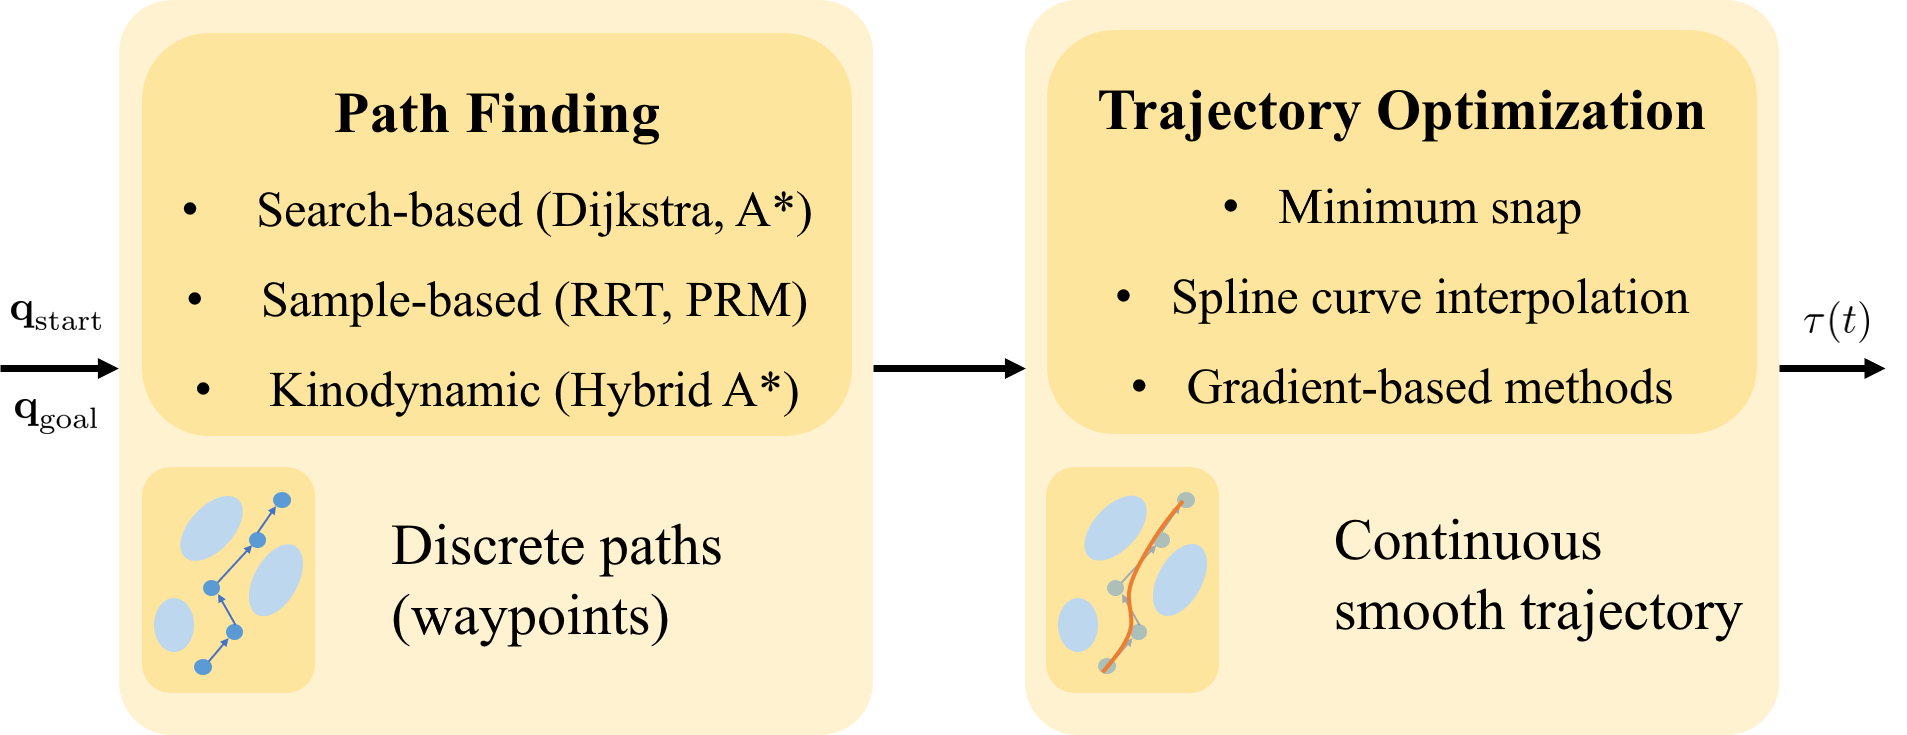
\includegraphics[width=.5\textwidth]{frontback.png}
  \caption{Hierarchical planning pipeline: The path-finding module 
finds a geometric collision-free path, and then trajectory
optimization module generates a continuous state-admissable and kinodynamically
feasible trajectory.}
  \label{fig:concept}
\end{figure}

Traditional planning and control frameworks are decoupled.
The path-planning (or motion-planning) module serves as a guide system 
for the low-level controller driving the robot's movement. 
This module needs to generate a geometrically 
collision-free and possibly kinodynamically feasible trajectory 
(or motion setpoints) for the low-level controller.
Then the low-level control module can use these motion 
setpoints to control the actuators on the robots to move.

The planning method usually consists of a hierarchical 
planning pipeline (Fig.~\ref{fig:concept}), a path-finding
and a trajectory-optimization module.
The path-finding problem is defined to 
find a path 
$
\tau : \left[0,1\right]\rightarrow \robotConfig_{\text{free}} 
$
such that  
$\tau(0) = \B{q}_{\text{start}} \in \robotConfig_{\text{free}}$ 
and
$\tau(1) = \B{q}_{\text{goal}} \in \robotConfig_{\text{free}}$, 
where $\robotConfig_\text{free}$ is the obstacle-free configuration space of the robot
\footnote{For UAVs, $\robotConfig_\text{free} \subset SE(3)$.}, 
and $\B{q}_{\text{start}}$ and $\B{q}_{\text{goal}}$ are the start and goal transformations, respectively.
The path $\tau$ can be a geometrically feasible discrete path.
To generate smooth trajectories with time profile 
for robots to 
follow based on discrete planned waypoints, the 
trajectory-optimization module is usually added to 
the pipeline. 
The control method aims to precisely command the 
UAV to track the given path (or trajectory), where 
general proportional-integral-derivative (PID) , 
robust, adaptive and optimal control methods may be utilized.


\section{Reinforcement Learning for Motion Planning \& Control}

In this section, we will discuss various RL algorithms for robotic 
motion planning and control, especially for UAV platforms. 
To ensure the coherency and consistency of the contents below, 
we adopt the following math representation: the states 
$\B{x}_t \in \boldsymbol{\mathcal{X}}$ 
and actions (inputs) $\B{u}_t \in \boldsymbol{\mathcal{U}}$ of a system (or an environment $\boldsymbol{\mathcal{E}}$) where $t\in\left[1,T\right]$ ($T$ may be $\infty$), 
the reward function $r(\B{x}_t, \B{u}_t)$, 
the initial state distribution $p(\B{x}_1)$, 
the transition probability $p(\B{x}_{t+1} | \B{x}_t, \B{u}_t)$, 
the policy $\pi(\B{u}_t | \B{x}_t)$, 
the return $G_t = \sum_{i=t}^T\gamma^{i-t}r(\B{x}_i, \B{u}_i)$ where $\gamma \in \left(0,1\right]$ is the discount factor, 
the value function $V(\B{x}_t) = \mathbb{E}\left[G_t | \B{x}_t\right]$, 
the action-value function $Q(\B{x}_t, \B{u}_t) = \mathbb{E}\left[G_t | \B{x}_t, \B{u}_t\right]$, 
and the goal is to maximize $G = \max \mathbb{E}\left[G_1 \right]$.

% Robot arm control has been a popular field for reinforcement learning 
% applications.
% \textcite{gu2017deep} propose an asynchronous off-policy update
% algorithm for DRL-based robotic manipulation, which utilizes
% the normalized advantage functions (NAF) proposed by 
% \textcite{gu2016continuous}.
% NAF parameterizes the advantage function into a quadratic form. 
% By introducing NAF, the Q function $Q(\B{x}_t, \B{u}_t)$ 
% in the continuous Q-learning can be represented in a way that
% the maximum, $\arg\max_{\B{u}_t}Q(\B{x}_t, \B{u}_t)$, can be determined 
% analytically during the Q-learning update.
% The Q function and the advantage function are represented as 
% \begin{equation}
% \label{eq:NAF}
% \begin{aligned}
%   Q(\B{x},\B{u}|\theta^Q) &= A(\B{x}, \B{u}|\theta^A) + V(\B{x}|\theta^V) \\
%   A(\B{x}, \B{u}|\theta^A) &=-\frac{1}{2} 
%   (\B{u} - \boldsymbol{\mu}(\B{x}|\theta^\mu))^\top
%   \B{P}(\B{x} | \theta^P)
%   (\B{u} - \boldsymbol{\mu}(\B{x}|\theta^\mu))
% \end{aligned}
% \end{equation}
% where $\theta^Q = \left\{ \theta^\mu, \theta^P, \theta^V \right\}$ is the 
% neural network parameters and $\B{P}(\B{x} | \theta^P)$ is a positive definite matrix.
% Therefore, $\arg\max_{\B{u}}Q(\B{x}, \B{u})$ is always given by
% $\boldsymbol{\mu}(\B{x} | \theta^\mu)$.
% In the robotic manipulation application, NAF is extended
% by asynchronous off-policy update using multiple threads (as in Algo.~\ref{algo:AsyncNAF})
% achieving better sample-efficacy.
% The asynchronous NAF algorithm is used to train a 7-DOF and the JACO arms 
% to perform tasks such as door pushing and pulling and pick and place.
% \begin{algorithm}[h]
%   \tcp{trainer thread}
%   Randomly initialize normalized Q network $Q(\B{x}, \B{u} | \theta^Q)$, where $\theta^Q = \left\{ \theta^\mu, \theta^P, \theta^V \right\}$\\
%   Initialize target network $Q^\prime$ with weight $\theta^{Q^\prime} \leftarrow \theta^Q$ \\
%   Initialize shared replay buffer $R \leftarrow \emptyset$ \\
%   \For{iteration=1,$I$} {
%     Sample a random minibatch of $m$ transitions from $R$ \\
%     Set 
%     $ y_i = 
%     \begin{cases}
%       r_i + \gamma V^\prime(x_i^\prime | \theta^{Q^\prime}) &\text{if}\quad t_i < T\\
%       r_i &\text{if}\quad t_i = T
%     \end{cases}
%     $\\
%     Update the weight $\theta^Q$ by minimizing the loss: 
%     $L = \frac{1}{m}\sum_i(y_i - Q(\B{x}_i, \B{u}_i))^2$ \\
%     Update the target network: 
%     $\theta^{Q^\prime} \leftarrow \tau \theta^{Q} + (1 - \tau)\theta^{Q^\prime}$
%   }
%   \tcp{collector thread $n,\;n=1,\dots,N$}
%   Randomly initialize policy network $\boldsymbol{\mu}(\B{x} | \theta_n^\mu)$ \\
%   \For{episode=1,$M$} {
%     Sync policy weight network $\theta_n^\mu \leftarrow \theta^\mu$ \\
%     Initialize a random process $\mathcal{N}$ for action exploration \\
%     Receive initial observation state $\B{x}_1 \sim p(x_1)$ \\
%     \For{t=1,T} {
%       Select action $\B{u}_t = \boldsymbol{\mu}(\B{x}_t | \theta_n^{\mu}) + \mathcal{N}_t$ \\
%       Execute $\B{u}_t$ and observe $r_t$ and $\B{x}_{t+1}$ \\
%       Send transition $(\B{x}_t, \B{u}_t, r_t, \B{x}_{t+1}, t)$ to $R$\\
%     }
%   }
%   \caption{Asynchronous NAF - N collector threads and 1 trainer thread}\label{algo:AsyncNAF}
% \end{algorithm}

Before diving into the recent work about RL in motion planning and 
control for quadrotors, we may first investigate this work proposed by 
\textcite{roy2002motion} on mobile robots.
In this early work, the motion planning method for the ground mobile robot 
generates a complete plan in the full state space of the robot, including orientation and velocity. 
It begins with an intermediate plan in a low-dimensional discrete space, using dynamic programming over a value function, and then projects this plan to the full state space. The plan is then refined through gradient ascent to increase the expected reward.
The state is defined as $\B{x}_t = \left[ x, y, \theta, v^t, v^r\right]^\top$ representing the $x$ and $y$ coordinates, orientation, linear 
and rotational velocities, respectively.
The action of this work is defined as $\B{u}_t = \left[ \Delta v^t, \Delta v^r \right]$.
The policy desired of this method is defined as a series 
of waypoints $\pi(\B{x}_i) = \left[ \B{w}_1, \dots, \B{w}_n\right]^\top$.
The value function in the matrix-vector form is defined as 
\[
  V(\pi_n) = \int_{t=0}^{T} G(\B{x}_t) R(\B{x}_t) dt 
           = \sum_{j=0}^{n-1} \int_{\B{x}(\B{w}_j)}^{\B{x}(\B{w}_{j+1})} G(\B{x}) R(\B{x}) dx 
\]
where $G(\cdot)$ is the state-transition matrix (this method
is model-based).
The algorithm for this method generating a series of waypoints is listed as in Algo.~\ref{algo:roy2002}.
\begin{algorithm}
  \caption{Motion planning through policy search}
  \label{algo:roy2002}

  Use value iteration to run the dynamic program and extract a policy from 2-dimensional value function \\

  Determine the maximum likelihood trajectory and convert to a set of 5-dimensional waypoints to form the expected path. \\

  \While{$\neg$ converged}
  {
    \ForEach{Waypoint $\B{w}_j$}
    {
      Determine value contribution of trajectory from previous waypoint $\B{w}_{j-1}$ to next waypoint $\B{w}_{j+1}$ \\
      Measure gradient at endpoints \\
      Move waypoint $\B{w}_j$ along gradient until path segment value increases \\
    }

    Find lowest immediate reward along the trajectory \\
    Insert a new waypoint
  }
\end{algorithm}
This method, though a good attempt utilizing the core idea from RL to motion planning, 
is constrained by the complex definitions and framework, making
it not common and practical for quadrotor planning and control.
Besides, the generated waypoint-like path is not continuous nor 
kinodynamically feasible for high-speed vehicle such as quadrotors.

Control methods such as model prediction control (MPC) need
explicit and accurate state estimations of the robot.
RL can release the agent from the strict constraint and 
directly map the raw sensor data to control inputs to the agent.
In the work of \textcite{zhang2016learning}, 
\begin{algorithm}
  \caption{Generic guided policy search summary}
  \label{algo:general_gps}
  \For{iteration i = 1 to K}
  {
    Optimize trajectory distributions $p_i(\tau)$ to minimize 
    $\mathbb{E}_{p_i}\left[l(\tau)\right]$ and deviation from 
    the policy $\pi_\theta(\B{u}_t | \B{o}_t)$ \\
    Generate samples $\left\{ \tau_i^j \right\}$ from each $p_i(\tau)$ \\
    Tain non-linear policy $\pi_\theta(\B{u}_t | \B{o}_t)$ to
    match the sampled trajectories $\left\{ \tau_i^j \right\}$ \\
    Update Lagrange multipliers to encourage agreement between
    $p_i(\B{u}_t | \B{x}_t)$ and $\pi_\theta(\B{u}_t | \B{x}_t)$
  }
\end{algorithm}
the authors propose to combine MPC with RL in the framework of guided policy search (GPS), where MPC is used to generate data at training time, under full state observations provided by an instrumented training environment.
Unlike common policy-gradient RL algorithms, the proposed GPS 
method uses a variant of differential dynamic programming (DDP), iterative
linear gaussian control (iLQG), usually applied in optimal 
control. 
The iLQG method is set as the guide to let the policy 
away from poor local minimal.
The general MPC-based GPS algorithm is illustrated in Algo.~\ref{algo:general_gps}, where $\tau = \left\{ \B{x}_1, \B{u}_1, \dots, \B{x}_T, \B{u}_T\right\}$ denotes the trajectory, 
$p(\tau) = p(\B{x}_1)\prod_{t=1}^{T}p(\B{x}_{t+1} | \B{x}_t, \B{u}_t)
\pi_\theta(\B{u}_t | \B{x}_t)$, 
$l(\tau) = \sum_{t=1}^T l(\B{x}_t, \B{u}_t)$, and 
$\pi_\theta(\B{u}_t | \B{x}_t) = \int \pi_\theta(\B{u}_t | \B{o}_t) p(\B{o}_t | \B{x}_t)d\B{o}_t$ 
($\B{o}_t$ is the observation).
Note that in this algorithm, the iLQG needs to know the approximate system
model of the quadrotor, so as to generate suitable guidance trajectories.
The non-linear policy $\pi_\theta(\B{u}_t | \B{o}_t)$ is trained 
using supervised learning from the samples collected via MPC.
With the assumption that the policy is Gaussian, i.e., 
$\pi_\theta(\B{u}_t | \B{o}_t) = \mathcal{N}(\mu^\pi(\B{o}_t), 
\Sigma^\pi(\B{o}_t))$, the training objective is the KL-divergence
\[
  \begin{aligned}
    D_\text{KL} & (
      \pi_\theta(\B{u}_t | \B{o}_t^{i,j} || 
      \tilde{p}_{i,j}(\B{u}_t | \B{x}_t^{i,j})) = \\
      &\frac{1}{2} (\mu^\pi(\B{o}_t) - \tilde{g}_{tij}(\B{x}_t))^\top
      \tilde{Q}_{\B{u},\B{u},tij}
      (\mu^\pi(\B{o}_t) - \tilde{g}_{tij}(\B{x}_t)) \\
      & -\frac{1}{2}\text{tr}\left[
        \tilde{Q}_{\B{u},\B{u},tij}\Sigma^\pi(\B{o}_t)
      \right]
      + \frac{1}{2}\log{\lvert \Sigma^\pi(\B{o}_t) \rvert}
      + \lambda^\top_{\mu,t}\mu^\pi(\B{o}_t)
  \end{aligned}
\]
where $\tilde{g}$ is the feedback control policy from iLQG.

In the experiments of \textcite{zhang2016learning}, the true state 
of the agent is $\B{x}_t = \left[ \B{p}_t, \B{v}_t, \B{q}_t, \boldsymbol{\omega}_t \right]^\top \in \mathbb{R}^{13}$.
The control input (action) $\B{u}_t \in \mathbb{R}^4$ is the 
rotor speed of the vehicle.
The observation model is $\B{o}_t = \left[ 
  \B{r}_t, \B{v}_t, \B{q}_t, \boldsymbol{\omega}_t 
\right] \in \mathbb{R}^{40}$  without the position $\B{p}_t$
instead including the reading $\B{r}_t$ from a set of 30 
equally spaced laser rangefinders with max range 5m arranged
in 180 degree fan in front of the vehicle.
Their experiments in the simulation show promising results 
for the quadrotor to perform simple object avoidance.
However, the demonstration shows significant input oscillations 
which make the quadrotor control not smooth.


In the guided policy search work \parencite{zhang2016learning}, 
there is a prior approximate quadrotor dynamics model for the 
MPC to generate guided trajectories.
The approach of \cite{hwangbo2017control} eliminates the need for predefined control structures, typically required in more traditional methods. 
Their new learning algorithm, which they claim is more suitable for quadrotor control than existing ones, is both conservative and stable for complex tasks. 
Their proposed approach is built on deterministic policy optimization using natural gradient descent adopted from trusted region policy optimization (TRPO).
The exploration strategy in the proposed method includes three types of 
trajectories: initial trajectories, junction trajectories and branch trajectories. The initial and branch trajectories are on-policy and the junction trajectories are off-policy generated with an additive Gaussian noise with covariance $\Sigma$. The branch trajectories are on-policy trajectories starting from some state along the junction trajectories.
Following an actor-critic fashion, the proposed method consists of a value and a policy network.
The value network is trained using Monte-Carlo samples 
obtained from on-policy trajectories, 
while the policy optimization utilizes both on-policy and 
off-policy trajectories.
The policy is trained as in Algo.~\ref{algo:policy_optimization} 
(superscripts $p$ and $f$ mean on-policy and off-policy, respectively).
\begin{algorithm}
  \caption{Policy optimization}
  \label{algo:policy_optimization}
  Give initial parameters of $V(\B{x} | \eta)$ and $\pi(\B{x} | \theta)$ \\
  \While{j = 1, 2, 3, $\dots$ until convergence}
  {
    Collect data using the three trajectories \\
    Compute the MC estimate of the value function:
    \[
      v_i = \sum_{t=i}^{T-1}\gamma^{t-i}r_t^p + \gamma^{T-i}V(\B{x}_T | \eta)
    \] \\
    Update $V(\B{x} | \eta)$ using Huber loss \\
    Update $\pi(\B{x} | \theta)$ using junction pairs (indexed with $k$) and natural gradient descent: 
    \[
      \begin{aligned}
        &&A^\pi(\B{x}_i, \B{u}_i^f) = r_i^f + \gamma v_{i+1}^f - v_i^p \\
        &&\bar{L}(\theta) = \sum_{k=0}^K A^\pi(\B{x}_k, \pi(\B{x}_k | \theta)) \\
        &&\theta_{j+1} \leftarrow  \theta_j - \frac{\alpha}{K}\sum_{k=0}^K n_k \\
        &\text{s.t.}&(\alpha n_k)^\top D_{\theta \theta}(\alpha n_k) < \delta, \forall k \\
        &&D_{\theta \theta} n_k = g_k
      \end{aligned}
    \]
  }
\end{algorithm}
The main task for the proposed method is to achieve stable waypoint
tracking.
During the operation, the input of the policy the subtracted 
by the waypoint location.
They also add a proportional and derivative (PD) controller 
\[
  \boldsymbol{\tau}_b = \B{k}_p  \B{R}^\top \B{q} + 
  \B{k}_d  \B{R}^\top\boldsymbol{\omega}
\]
for the attitude along with the learning policy, 
where $\boldsymbol{\tau}_b$ is the virtual torque on the main 
body, $\B{q}$ and $\B{R}$ are the orientation of the quadrotor in Euler
vector and rotation matrix forms respectively, and $\boldsymbol{\omega}$
is the angular velocity.
The sum of the PD controller and the learned policy is used 
as the command.
The reward function is defined as 
\[
  r_t = 4\times 10^{-3} \lVert \B{p}_t \rVert  + 
    2 \times 10^{-4} \lVert \B{a}_t \rVert + 
    3 \times 10^{-4} \lVert \boldsymbol{\omega}_t \rVert + 
    5 \times 10^{-4} \lVert \B{v}_t \rVert
\]
In the experiments, they perform both simulations and real-world
experiments. The trained policy shows great performance and 
remains computationally cheap at the same time. 
The computation time of evaluating the policy is only 7 $\mu$s
per time step, which is two orders of magnitude less than common
trajectory optimization algorithms with an approximate model.

Autonomous drone racing is a popular robotics task for the 
quadrotor traveling through a set of waypoints as fast as possible. 
\textcite{song2021autonomous} propose an approach
using deep reinforcement learning to train the quadrotor 
traversing aggressively between gates in the drone racing task.
The main contribution of this work is the novel reward settings 
and the randomization techniques used for training.
To fast and safely travel through gates, the reward function is divided into
two main parts: the progress part and the safety part.
The progress reward is a positive reward for the quadrotor to pass
the gates.
The position of the quadrotor is projected onto the current line 
segment between the previous gate and the next gate to be passed.
Given the current position $\B{p}_c(t)$ and the previous position 
$\B{p}_c(t-1)$ of the quadrotor, the progress reward $r_{{p}}(t)$is defined as 
\[
  r_{{p}}(t) = s(\B{p}_c(t)) - s(\B{p}_c(t-1))
\]
where $s({p}) = (\B{p} - \B{g}_1) \cdot (\B{g}_2 - \B{g}_1) / \lVert (\B{g}_2 - \B{g}_1) \rVert$ defining the progress along the path
segment that connects the previous gate's position $\B{g}_1$ 
with the next gate's position $\B{g}_2$.
The safety reward is defined as: 
\[
  r_{s} = - f^2 \cdot \left(
    1 - \exp\left(- \frac{d_n^2}{2v}\right)
  \right)
\]
where $f = \max\left[1 - (d_p / d_{\max}), 0.0\right]$
and $v = \max\left[ (1-f)\cdot(w_g/6), 0.05 \right]$.
Here, $d_n$ and $d_p$ denote the distance of the quadrotor 
to the gate normal and the distance to the gate plane respectively.
The final reward ad each time step $t$ is 
\[
  r(t) = r_{p}(t) + a \cdot r_s(t) - b \cdot \lVert \boldsymbol{\omega} \rVert^2 + 
  \begin{cases}
    r_T & \text{if gate collision} \\
    0 & \text{else}
  \end{cases}
\]
where $r_T$ is a terminal reward for penalizing the gate collisions
$r_T = -\min\left[\left(\frac{d_g}{w_g}\right)^2, 20.0\right]$
with $d_g$ and $w_g$ denoting the euclidean distance from the 
position of the crash to the gate center and the side length 
of the rectangular gate, respectively.
The observation space is divided into two main components, including 
the quadrotor's state $\B{x}_t^{\text{quad}}$ and the tracking information
$\B{x}_t^{\text{track}}$.
The quadrotor state is 
\[\B{x}_t^{\text{quad}} = \left[
  \B{v}_{WB,t}, \;
  \dot{\B{V}}_{WB,t}, \;
  \B{R}_{WB,t}, \;
  \boldsymbol{\omega}_{B,t}
\right] \in \mathbb{R}^{18}
\]
The track observation vector $\B{x}_t^{\text{track}}$
is defined as 
\[
  \B{x}_t^{\text{track}} = \left[
    \B{o}_1, \;
    \alpha_1, \;
    \dots, \;
    \B{o}_i, \;
    \alpha, \;, 
    \dots
  \right], 
  i\in\left[1,\dots,N\right]
\]
where $\B{o}_i \in \mathbb{R}^3$ denotes the observation for 
gate $i$ and $N\in\mathbb{Z}^+$ is the total number of future
gates.
The observation for the gate use spherical coordinates 
$\B{o}_i = \left(p_r, p_\theta, p_\phi\right)_i$.
The angle between the gate normal and the vector pointing from the 
quadrotor to the center of gate $i$ is denoted as $\alpha_i \in \mathbb{R}$.
The action in this work is directly mapped to the rotor 
thrust commands, i.e., $\B{u}_t = \left[ f_1, f_2, f_3, f_4 \right]$.

In the policy training of \textcite{song2021autonomous}, the authors
use Proximal Policy Optimization (PPO) algorithm. 
Due to the high dimensionality of the search space, they use several techniques to accelerate the training speed:
\begin{itemize}
  \item Parallel Sampling Scheme: Utilizes simulation to simultaneously perform policy rollouts in up to 100 environments. This speeds up data collection and enhances the diversity of environmental interactions, allowing coverage of entire race tracks and preventing overfitting to specific track configurations.
  \item Distributed Initialization Strategy: Addresses initial gate crashes by randomly placing quadrotors in hover states around all path segments. This strategy ensures uniform exploration of the state space and is refined as the policy improves, leading to more effective exploration.
  \item Random Track Curriculum: Handles the increased complexity when training with randomly sampled race tracks. A track generator creates tracks of varied complexity and length. The training process adapts the complexity of tracks based on the agent's performance, starting with simpler tracks and progressing to more complex ones as the agent's ability to navigate gates improves. This approach maintains a focus on minimizing lap times in diverse track environments.
\end{itemize}




\section{Discussions and Conclusion}

The preceding section offers an insightful but not exhaustive overview of motion planning and control for quadrotors using reinforcement learning (RL) methods. It suggests that data-based RL methods can sometimes outperform traditional approaches.

Traditional trajectory optimization and control theory have a long history, providing well-defined mathematical formulations for quadrotor dynamics and trajectory generation. However, these model-driven methods often yield sub-optimal results due to the inherent stochastic nature of the physical world and the impossibility of perfect models. Additionally, the increasing complexity of tasks, such as high-speed drone racing, poses further challenges to traditional methods.

In contrast, data-driven RL methods have shown promising results in various robotics applications, contributing to the development of more versatile and robust systems. However, the author of this survey would propose two main challenges in the motion planning anc control field for RL:
\begin{itemize}
  \item Guaranteed Safety: Ensuring consistent safety in RL applications is a critical issue that needs addressing. 
  \item Action Smoothness: Achieving smooth and consistent actions in RL-based control systems is another challenge that requires attention.
\end{itemize}

Many research studies demonstrate the significant potential of integrating traditional methods with RL techniques to enhance motion planning and control solutions. In the future, merging the mathematical foundations of traditional approaches with the data-driven insights of RL methods will generate more robust and effective systems.

\printbibliography

\end{document}